\section {Results}
\label{results}

\subsection {Analysis} 
%Since $H_{1}$ concerns the mean count of xyz for each word, a one-tailed Student's Independent \textit{t}-test will be used here to determine whether the mean count of xyz for nouns are statistically significantly greater than those for adjectivs.  The threshold for significance adopted here is $0.01$.  

\subsection{Total MAE (Error Over All Imitation Types)}
Figure \ref{fig:overall} shows the overall error for each variation of the genetic algorithm. Overall, the best algorithm was algorithm 1 with an MAE of $184.89$ while the worst, algorithm 8, had an MAE of $188.82$. Since the genetic alignment algorithms are all deterministic in nature, these errors are always the same. Subsequently, their standard deviation is 0 and their average is what they are. This makes them statistically significantly different. Thus, with $p < 0.00...01$, algorithm 1 is better than all other algorithms thus far demonstrated.

\begin{figure}[center]
	\centering
	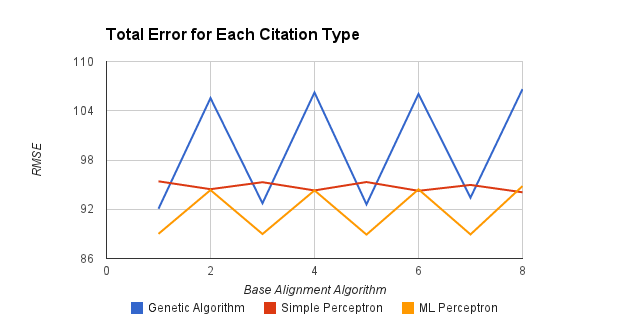
\includegraphics[width=16cm]{images/error_type_all_imitations.png}
	\caption{Note that genetic alignment outperformed baseline in all cases.}
	\label{fig:overall}
\end{figure}

\subsection{Error By Imitation Class}
Figures \ref{fig:c1}-\ref{fig:6} demonstrate that the various versions of genetic alignment behave differently. This is expected behavior: Their preferences cause them to be more adept for certain imitation classes. The best genetic algorithm for each class is given in table \ref{tab:best-for-each}.

\begin{table}[center]
	\centering
	\begin{center}
		\begin{tabular}{|l|c|c|} \hline
			\textbf{Imitation Type}	& \textbf{Best Algorithm}	&	\textbf{Error (MAE)}	\\ \hline \hline
			1						& 1							&	147.08					\\ \hline
			2						& 2							&	272.56					\\ \hline
			3						& 1							&	161.01					\\ \hline
			4						& 1							&	271.10					\\ \hline
			5						& 1							&	183.64					\\ \hline
			6						& 1							&	182.76					\\ \hline
		\end{tabular}
	\end{center}
	\caption{Algorithm 1 has the best MAE for $6/7$ of the imitation types.}
	\label{tab:best-for-each}
\end{table}

Interestingly, algorithm 1 is often the best algorithm. Subsequently, this is also true for the MAE over all imitation types. Algorithm 1 combined wih BP-MLP ends up being the best high-order combinational model. However, in when simple linear regression is used, algorithm 1 ends up being the worst model.

\begin{figure}[center]
	\centering
	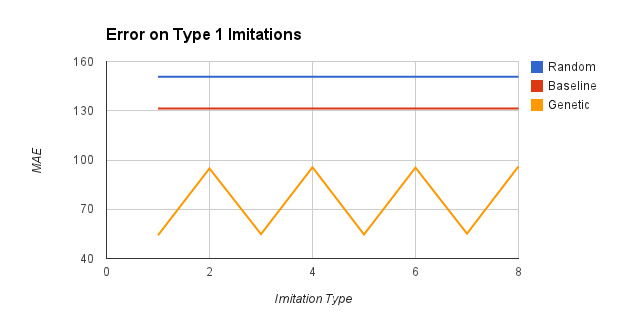
\includegraphics[width=16cm]{images/error_type_1_imitations.png}
	\caption{}
	\label{fig:c1}
\end{figure}
\begin{figure}[center]
	\centering
	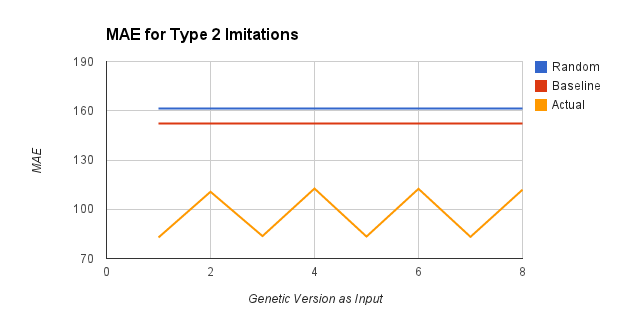
\includegraphics[width=16cm]{images/error_type_2_imitations.png}
	\caption{}
	\label{fig:c2}
\end{figure}
\begin{figure}[center]
	\centering
	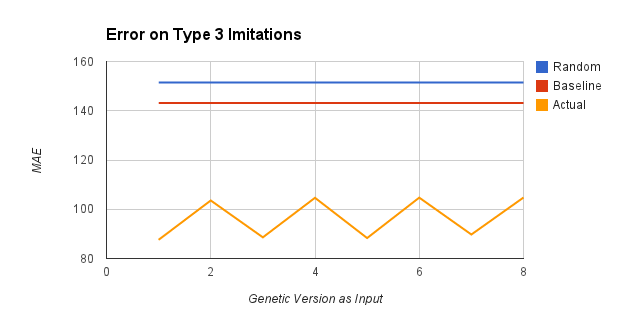
\includegraphics[width=16cm]{images/error_type_3_imitations.png}
	\caption{}
	\label{fig:c3}
\end{figure}
\begin{figure}[center]
	\centering
	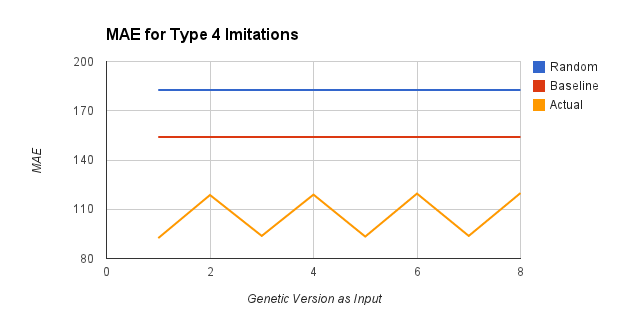
\includegraphics[width=16cm]{images/error_type_4_imitations.png}
	\caption{}
	\label{fig:c4}
\end{figure}
\begin{figure}[center]
	\centering
	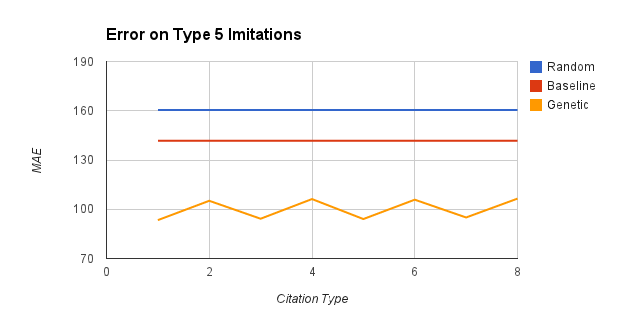
\includegraphics[width=16cm]{images/error_type_5_imitations.png}
	\caption{}
	\label{fig:c5}
\end{figure}
\begin{figure}[center]
	\centering
	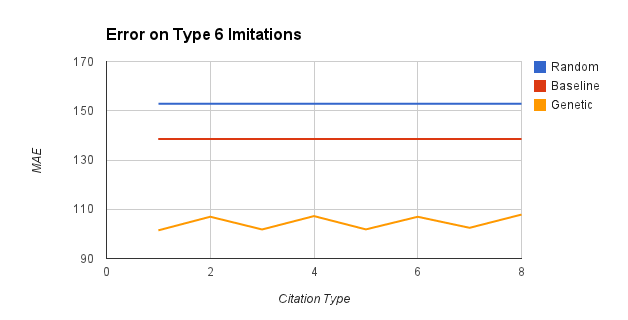
\includegraphics[width=16cm]{images/error_type_6_imitations.png}
	\caption{}
	\label{fig:c6}
\end{figure}

%\subsection{Best in Each Category}
%Figures xyz %~\ref{theoreticalCombinedError} 
%shows the lowest error achieved for each imitation type.

\clearpage

\subsection{BP-trained MLP Performance}
(xyz fill this in)

\begin{figure}[center]
	\centering
	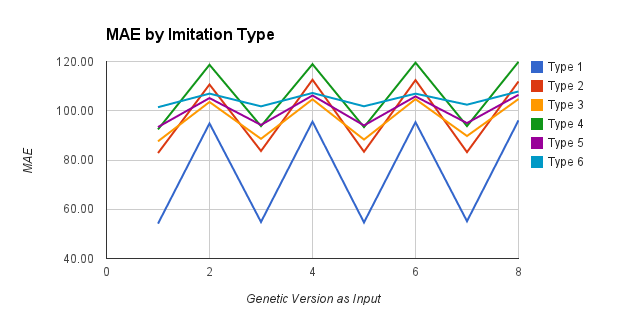
\includegraphics[width=16cm]{images/total_error_all_approaches.png}
	\caption{Regression provided by machine learning trumps the errors for genetic alignment. Furthermore, higher-ordered BP-MLP models provide the lowest errors.}
	\label{fig:overall_ml}
\end{figure}

It is 
\begin{figure}[center]
	\centering
	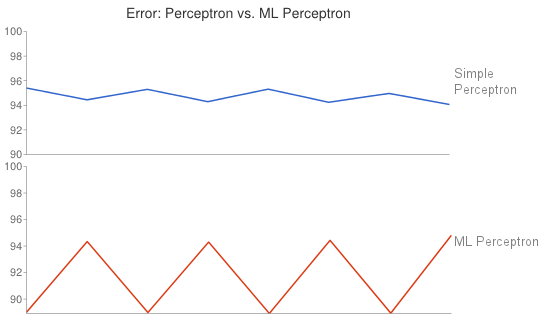
\includegraphics[width=12cm]{images/Perceptron_vs_ML.png}
	\caption{An interesting correlation that lows in perceptron are highs in BP-MLP.}
	\label{fig:perceptron_vs_bp}
\end{figure}
\clearpage

%%%%%%%%%%%%%%%%%%%%%%%%%%%%%%%%%%%%
%sample helps from previous research
%%%%%%%%%%%%%%%%%%%%%%%%%%%%%%%%%%%%

%\begin{table}
	\begin{center}
		\begin{tabular}{|c|c|c|c|c|} \hline
			\textit{HOT} & \textit{BLACK} & \textit{TALL} & \textit{LARGE} & \textit{UGLY} \\ \hline \hline
			cold	&	white	&	short	&	small	&	pretty		\\
			cold	&	white	&	short	&	small	&	beautiful		\\
			cold	&	white	&	short	&	tiny	&	beautiful		\\
			cold	&	white	&	short	&	small	&	beautiful		\\
			not hot	&	not black	&	not tall	&	not large	&	not ugly		\\
			cold	&	white	&	short	&	small	&	pretty		\\
			cold	&	light	&	short	&	petite	&	pleasing		\\
			cold	&	white	&	short	&	small	&	beautiful		\\
			frigid	&	white	&	short	&	miniscule	&	breathtaking		\\
			ugly	&	white	&	short	&	small	&	pretty		\\
			cold	&	white	&	short	&	small	&	pretty		\\
			cold	&	white	&	short	&	small	&	pretty		\\
			cold	&	white	&	short	&	small	&	beautiful		\\
			cold	&	white	&	short	&	small	&	pretty		\\
			cold	&	white	&	short	&	small	&	beautiful		\\
			cold	&	white	&	short	&	small	&	pretty		\\
			cold	&	white	&	short	&	small	&	pretty		\\
			cold	&	white	&	short	&	small	&	beautiful		\\
			cold	&	white	&	short	&	small	&	Beauty 		\\
			cold	&	white	&	short	&	small	&	pretty		\\
			cold	&	white	&	short	&	small	&	beautiful		\\
			cold	&	white	&	short	&	small	&	pretty		\\
			cold	&	white	&	short	&	small	&	beautiful		\\
			cold	&	N/A	&	N/A	&	N/A	&	beautiful		\\
			cold	&	white	&	short	&	small	&	beautiful		\\
			cold	&	mirrored	&	short	&	small	&	beautiful		\\
			freezing	&	N/A	&	N/A	&	insignificant	&	N/A		\\
			cold	&	white	&	short	&	small	&	beautiful		\\
			cold	&	light	&	diminutive	&	petite	&	exquisite		\\
			cold	&	white	&	short	&	small	&	beautiful		\\
			cold	&	white	&	short	&	small	&	pretty		\\
			cold	&	white	&	short/small	&	small	&	pretty		\\
			%cold	&	white	&	short	&	small	&	beautiful		\\
			%cold	&	white	&	short	&	small	&	beautiful		\\
			cold	&	white	&	short	&	small	&	pretty		\\ \hline
			%sexless	&	white	&	short	&	diminished	&	kind		\\ 
			\textbf{6}	&	\textbf{5}	&	\textbf{5}	&	\textbf{7}	&	\textbf{8}		\\
			\hline
		\end{tabular}
	\end{center}
	\caption {All antonym responses for each adjective with total number of unique responses.}
	\label{tab:all_adjective}
\end{table}

\begin{table}
	\begin{center}
		\begin{tabular}{|c|c|c|c|c|} \hline
			\textit{ZIPPER} & \textit{SKY} & \textit{SHOE} & \textit{ROBOT} & \textit{CARPET} \\ \hline \hline
			Velcro	&	ground	&	glove	&	human	&	hard floor		\\
			button(s)	&	Earth	&	glove	&	living being	&	hard floor		\\
			Velcro	&	ground	&	sock(s)	&	Free	&	ceiling		\\
			lace(s)	&	ground	&	glove	&	human	&	ceiling		\\
			not zipper	&	not sky	&	not a shoe	&	not robot	&	not carpet		\\
			button(s)	&	ground	&	sock(s)	&	human	&	ceiling		\\
			razor	&	dirt	&	hat	&	sentient being	&	canopy		\\
			button(s)	&	ground	&	barefeet	&	human	&	tile		\\
			button(s)	&	Earth	&	barefeet	&	human	&	tile		\\
			button(s)	&	ground	&	sock(s)	&	human	&	tile		\\
			unzipper	&	ground	&	barefeet	&	organic/organism	&	ceiling		\\
			button(s)	&	Earth	&	barefeet	&	person	&	hardwood		\\
			button(s)	&	ground	&	barefeet	&	human	&	hardwood		\\
			button(s)	&	land	&	sock(s)	&	human	&	tile		\\
			button(s)	&	ground	&	sock(s)	&	organic/organism	&	tile		\\
			button(s)	&	ground	&	hat	&	human	&	wood		\\
			N/A	&	Earth	&	N/A	&	person	&	tile		\\
			button(s)	&	Earth	&	sandal	&	human	&	hardwood		\\
			Unzip	&	Earth	&	barefeet	&	human	&	hardwood		\\
			button(s)	&	ground	&	glove	&	person	&	hardwood		\\
			button(s)	&	ground	&	barefeet	&	baby	&	ceiling		\\
			ripper	&	hell	&	glove	&	human	&	hardwood		\\
			scissors	&	ground	&	hat	&	grass	&	ceiling tiles		\\
			N/A	&	N/A	&	N/A	&	rock	&	ceiling		\\
			button	&	ground	&	foot	&	human	&	air		\\
			button	&	earth	&	hat	&	ghost	&	ceiling		\\
			N/A	&	land	&	N/A	&	N/A	&	N/A		\\
			antizipper	&	ground	&	glove	&	antirobot	&	anticarpet		\\
			snaps	&	ground	&	barefeet	&	organic	&	tile		\\
			velcro 	&	floor	&	barefeet	&	human	&	tile		\\
			velcro	&	earth	&	sandal	&	human	&	wood		\\
			button(s)	&	ground	&	slipper	&	human	&	concrete		\\
			%button(s)	&	ground	&	barefeet	&	person	&	wood		\\
			%button(s)	&	ground	&	barefeet	&	human	&	wood		\\
			button(s)	&	Ground	&	hat	&	Human	&	Dirt		\\ \hline
			%zip him	&	Earth	&	barefeet	&	human	&	ambulatory pet		\\ 
			\textbf{14}	&	\textbf{8}	&	\textbf{8}	&	\textbf{13}	&	\textbf{12}		\\
			\hline
		\end{tabular}
	\end{center}
	\caption {All antonym responses for each noun with total number of unique responses.}
	\label{tab:all_noun}
\end{table}


%The Welch's \textit{t}-test agrees that there is significance (equal variance not assumed):%
%	\begin{quote}
%		$t(5)=4.1642, p < 0.00439413$
%	\end{quote}

%\subsection{}
%Since there were few responses from men (only 9), it seems that running the same \textit{t}-test on the responses without the male responses could be of interest as well.  Tables~\ref{tab:female_adjective}, \ref{tab:female_noun} show the normalized responses and total counts for each set of xyz while Table~\ref{tab:female_group_stats} shows the group statistics for the two groups.


%The calculated statistic is as follows (equal variance not assumed):
%$t(7.881)=3.55902, p < 0.00461577$ 
